\chapter{Przedstawienie problemu od strony technicznej}
\label{cha:przedstawienieProblemuOdStronyTechnicznej}

\par Przedstawione zagadnienie, jest problemem złożonym. Można je rozdzielić (zgodnie z strategią \emph{Divide \& Conquer}) na kilka kategorii: komunikacja z użytkownikiem i innymi narzędziami informatycznymi, tworzenie i uruchamianie sparametryzowanych symulacji, przechowywanie danych bez określonego uprzednio typu oraz bezpieczeństwo i ryzyka związane z uruchamianiem kodu nieznanego pochodzenia.

\section{API jako interfejs dla Aplikacji Webowej}

\par Podejście do tworzenia oprogramowania bardzo się zmieniło w przeciągu ostatnich dziesięciu lat. Głównie za sprawą rozwoju infrastruktury sieciowej, zapewniającej dostęp do lepszej jakości połączenia internetowego użytkownikom, jak i ogromy wzrost popularności urządzeń mobilnych sprawił, że niegdyś dominująca forma tworzenia aplikacji, to znaczy aplikacje desktopowe, ustąpiły na rzecz usług czysto webowych, lub lekkich klientów które służą wyłącznie jako interfejs graficzny do interakcji z oprogramowaniem działającym na serwerze.

\begin{figure}[H]
	\begin{center}
		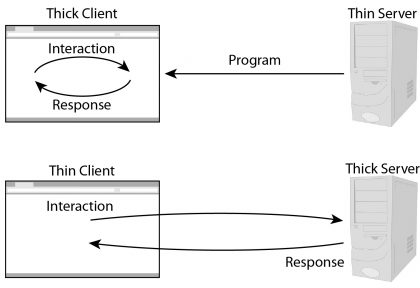
\includegraphics{Thick Thin Client}
	\end{center}
	\caption{Lekki i obszerny klient}
	\source{http://www.exe.com.pl/plusy-i-minusy-cienkiego-klienta/}
\end{figure}

Rozwiązanie to pozwala na o wiele większą swobodę w tworzeniu GUI \footnote{\emph{Graphical User Interface}}, które poprzez wykorzystywanie elementów graficznych często jest mocno związane z platformą na jakiej działa.

\par Dzięki rozdzieleniu tych dwóch elementów, możliwe jest stworzenie lekkiego klienta, na wybranej platformie (tak długo jak posiada ona dostęp do internetu oraz obsługuje protokół \texttt{\https{}}). Aplikacja graficzna, która wykorzystuje takie rozwiązanie jest bardzo lekka (brak konieczności dołączania dodatkowego oprogramowania np. serwera bazy danych), dzięki czemu nadaje się do działania na platformach mobilnych i/lub w przeglądarce, co z kolej prowadzi do zwiększenia potencjalnej liczby odbiorców naszego oprogramowania. Po drugiej stronie znajduje się natomiast API \footnote{\emph{Application Programming Interface}}, pełniący rolę serwera. Aplikacje klienckie łączą się z nim w celu wykonywania poszczególnych żądań, jak i uzyskania danych.

\par Warto wspomnieć o dodatkowych korzyściach płynących z takiego rozwiązania, mianowicie o \emph{Cloud Computing}u. Separacja głównej logiki aplikacji od urządzeń użytkowników pozwala na posiadanie niewielkich wymagań sprzętowych wobec nich, jak i wykorzystanie serwerów o dużej mocy obliczeniowej, które przy odpowiednim \emph{Load Balancing}u mogą zostać wykorzystane w pełni.

\section{Symulacje}

\par Symulacje komputerowe są tworzone w różnych celach. Przy ich pomocy inżynierowie mogą próbować określić wytrzymałość mostu, testować aerodynamikę samolotu lub przewidywać jak zmieni się ruch w mieście, gdy zamkniemy jedną ulicę na czas remontu, naukowcy mogą symulować ruch ciał niebieskich lub tworzyć prognozy rozprzestrzeniania się choroby w zależności od różnych zmiennych, a nauczyciele prezentować wizualizacje zjawisk fizycznych uczniom. Do tego symulacje dzielą się na dyskretne jak i ciągłe w czasie, deterministyczne i stochastyczne\cite{mchaney1991computer} lub lokalne i rozproszone. Zagadnienie to jest bardzo złożone i obsłużenie wszystkich przypadków jest niezwykle trudne.

\par Chcąc zapewnić jak największą swobodę użytkownikom, jak i mając na uwadze bezpieczeństwo naszego systemu trzeba ustalić pewne ograniczenia i kompromisy. Zdefiniowanie pewnego wspólnego interfejsu jest konieczne, aby zapewnić komunikację z instancją danej symulacji, w celu uruchomienia jej z ustalonymi parametrami, ale też by wyniki takiej symulacji zebrać i zachować do późniejszej prezentacji.

\par W celu zapewnienia odpowiedniego poziomu bezpieczeństwa, rozsądnym działaniem jest odcięcie takowej symulacji od internetu. To niestety wyklucza symulacje rozproszone z oczywistych przyczyn.

\section{Uruchamianie kodu \emph{3\textsuperscript{rd}-party}}

\par Bezpieczeństwo jest jednym z podstawowych zagadnień dla prawie każdego systemu komputerowego. Istnienie niedoskonałości w tej warstwie, w postaci podatności na ataki potrafi narazić na bezpieczeństwo zarówno użytkowników jak i samych twórców oprogramowania. Jedną z najbardziej niebezpiecznych czynności jakie może wykonać osoba korzystająca z internetu, jest uruchomienie oprogramowania nieznanego pochodzenia. Takowy software może robić wszystko, w tym dążyć do wycieku danych użytkowników, jak i doprowadzić do awarii całego systemu.

\par Do ograniczenia szkodliwych możliwości takiego oprogramowania, można wykorzystać wiele technik, np. zastosować odpowiednie prawa dostępu w systemie \emph{Linux}. Jednak najbezpieczniejszym rozwiązaniem jest całkowita izolacja takiego kodu, poprzez uruchomienie go w izolowanym środowisku, tak zwanym \emph{sandbox}ie. Pozwala to skutecznie zniwelować wszelkie szkody, które powstałyby w wyniku nieporządnego działania oprogramowania \emph{3\textsuperscript{rd}-party}.

\par Poza bezpieczeństwem ważny jest również sposób w jaki będziemy uruchamiać dostarczony nam kod. Oczywistym jest to, że pliki dostarczone przez użytkownika muszą być kompatybilne z środowiskiem w jakim będziemy chcieli je uruchomić. Jednak gdyby użytkownicy dostarczali nam gotowe programy (skompilowane do plików wykonywalnych (\emph{executable})), to istnieje że będą one korzystały z pewnych zależności (\emph{dependencies}), których nie będziemy posiadać. Kolejną kwestią istotną do rozważenia jest architektura pod jaką kod może zostać skompilowany (\texttt{x64}, \texttt{x86}, \texttt{ARM}). Programy dostarczone w tej formie mają jeszcze jedną poważną wadę - niemożliwość przetestowania ich zawartości, zgodności z ustalonym przez nas standardem. O ile nie umówilibyśmy się z użytkownikiem, na pewien rodzaj interfejsu (a nawet wtedy), sprawdzenie działania i zgodności danego programu mogłoby okazać się dużym wyzwaniem. Innym możliwym podejściem do tego problemu jest wymaganie dostarczenia kodu w postaci biblioteki (np. w jako plik \texttt{.JAR} lub \texttt{.DLL}) spełniającej udostępniony wcześniej standard.

\section{Przechowywanie danych}

\par O ile samo przechowywanie danych może wydawać się tematem trywialnym z perspektywy tworzenia oprogramowania w dobie istnienia bibliotek (a nawet całych \emph{framework}ów) zajmujących się zagadnieniem zapisu i odczytu danych, co pozwala na łatwe i szybkie projektowanie systemów (np. wykorzystując podejście \emph{Code First}). Zagadnienie to niestety komplikuje się w sytuacji nieznajomości typów danych jakie może chcieć przechowywać użytkownik.

\par Potencjalnym rozwiązaniem tego problemu jest serializacja danych. Proces ten polega na sprowadzeniu struktury przechowującej pewne informacje do formy przejściowej (np. pliku lub łańcucha znaków), na podstawie której można będzie w przyszłości odtworzyć pierwotny obiekt.

\par Inną kwestią o jakiej warto jest w tym miejscu wspomnieć jest przechowywanie plików przesłanych przez użytkowników, czyli tak zwanych BLOBów \footnote{\emph{Binary Large Object}}. Aby zapisać taki plik do bazy danych, należy go przekonwertować do postaci binarnej (tablicy bajtów) i w tej formie zapisać. Chcą skorzystać w przyszłości z tego pliku, należałoby odwrócić cały ten proces, co może negatywnie wpłynąć na wydajność naszej aplikacji, jak i na szybkość działania samej bazy danych. Popularnym rozwiązaniem tego problemu jest przechowywanie plików na dysku w formie niezmienionej i przetrzymywanie jedynie ścieżki dostępu lub skorzystanie z zewnętrznego serwisu specjalizującego się w obsłudze BLOBów.